%%%%%%%%%%%%%%%%%%%%%%%%%%%%%%%%%%%%%%%%%
% Thin Sectioned Essay
% LaTeX Template
% Version 1.0 (3/8/13)
%
% This template has been downloaded from:
% http://www.LaTeXTemplates.com
%
% Original Author:
% Nicolas Diaz (nsdiaz@uc.cl) with extensive modifications by:
% Vel (vel@latextemplates.com)
%
% License:
% CC BY-NC-SA 3.0 (http://creativecommons.org/licenses/by-nc-sa/3.0/)
%
%%%%%%%%%%%%%%%%%%%%%%%%%%%%%%%%%%%%%%%%%

%----------------------------------------------------------------------------------------
%   PACKAGES AND OTHER DOCUMENT CONFIGURATIONS
%----------------------------------------------------------------------------------------

\documentclass[a4paper, 11pt]{article} % Font size (can be 10pt, 11pt or 12pt) and paper size (remove a4paper for US letter paper)

\usepackage{hyperref}
\usepackage[portuguese,english]{babel}
\usepackage[utf8]{inputenc}
\usepackage{float}

\usepackage{color} % for the notes
\usepackage{xcolor}
\usepackage[protrusion=true,expansion=true]{microtype} % Better typography
\usepackage{graphicx} % Required for including pictures
\usepackage{wrapfig} % Allows in-line images
\usepackage{tocloft}
\usepackage{multirow}

\usepackage{mathpazo} % Use the Palatino font
\usepackage[T1]{fontenc} % Required for accented characters
\linespread{1.05} % Change line spacing here, Palatino benefits from a slight increase by default
\usepackage{etoolbox}
\newcommand{\firefox}{\textsc{f}irefox}
\newcommand{\floss}{\textsc{floss}}
\newcommand{\openoffice}{\textsc{o}pen\textsc{o}ffice}
\newcommand{\puredata}{\textsc{p}uredata}
\newcommand{\wiki}{\textsc{w}iki}
\newcommand{\etherpad}{\textsc{e}therpad}
\newcommand{\irc}{\textsc{irc}}
\newcommand{\ocd}{\textsc{ocd}}
\newcommand{\participa}{\textsc{p}articipa.br}
\newcommand{\httpb}{\textsc{http}}
\newcommand{\html}{\textsc{html}}
\newcommand{\nlp}{\textsc{nlp}}
\newcommand{\sectionb}{\textsc{s}ection}
\newcommand{\cn}{\textsc{cn}}
\newcommand{\aab}{\textsc{aa}}
\newcommand{\aai}{\textsc{Aa}}
\newcommand{\ontologiaa}{\textsc{o}ntologi\textsc{aa}}
\newcommand{\owl}{{\sc owl}}
\newcommand{\rdfi}{{\sc Rdf}}
\newcommand{\mongodb}{{\sc m}ongo{\sc db}}
\newcommand{\mysql}{{\sc m}y{\sc sql}}
\newcommand{\rdf}{{\sc rdf}}
%\newcommand{\paaineli}{P{\sc aa}inel}
\newcommand{\paaineli}{P{\bf \sc aa}inel}
\newcommand{\paainel}{p{\sc aa}inel}
\newcommand{\gsd}{\textsc{gsd}}
\newcommand{\ui}{\textsc{ui}}
%\newcommand{\lmb}{\url{lab\textsc{M}acambira.sf.net}}
\newcommand{\lm}{lab\textsc{M}acambira.sf.net}
%\newcommand{\lm}{\url{labMacambira.sf.net}}



\makeatletter
\renewcommand\@biblabel[1]{\textbf{#1.}} % Change the square brackets for each bibliography item from '[1]' to '1.'
\renewcommand{\@listI}{\itemsep=0pt} % Reduce the space between items in the itemize and enumerate environments and the bibliography

\hypersetup{
        colorlinks,
            linkcolor={red!50!black},
                citecolor={blue!50!black},
                    urlcolor={blue!80!black}
                }


\pretocmd{\chapter}{\addtocontents{toc}{\protect\addvspace{5\p@}}}{}{}
\pretocmd{\section}{\addtocontents{toc}{\protect\vspace{-4mm}}}{}{}
\renewcommand{\maketitle}{ % Customize the title - do not edit title and author name here, see the TITLE block below
\begin{flushright} % Right align
{\LARGE\@title} % Increase the font size of the title

\vspace{50pt} % Some vertical space between the title and author name

{\large\@author} % Author name
\\\@date % Date

\vspace{40pt} % Some vertical space between the author block and abstract
\end{flushright}
}

%----------------------------------------------------------------------------------------
%   TITLE
%----------------------------------------------------------------------------------------

\title{\textbf{The Algorithmic-Autoregulation essay}\\ % Title
%a natural collective focus\\on the collective being} % Subtitle
a collective and natural focus\\ on self-transparency} % Subtitle

\author{\textsc{Renato Fabbri} % Author
\\{\textit{IFSC/USP, Participa.br/SG-PR, labMacambira.sf.net}}} % Institution

\date{\today} % Date

%----------------------------------------------------------------------------------------

\begin{document}

\maketitle % Print the title section

%----------------------------------------------------------------------------------------
%   ABSTRACT AND KEYWORDS
%----------------------------------------------------------------------------------------

%\renewcommand{\abstractname}{Summary} % Uncomment to change the name of the abstract to something else


\begin{abstract}
    There are numerous pursues for a lightweight and systematic account of what is done by a group and containing individuals. The Algorithmic-Autoregulation (\aab) is a special case, in which a technical community embraced the challenge of registering their own dedication for sharing processes, self-transparency enhancements, and prove dedication. \aai\ is used since June/2011 by dozens of \floss\ and social developers, with the support of different \aab\ software gadgets and for distinct tasks. Intermittence and activity concentration of users activity follows expected natural properties. Social participation and ontological understandings of \aab\ eases comparative analysis and furthers integration.
\end{abstract}

{
\selectlanguage{portuguese}
\begin{abstract}

\end{abstract}
}

\hspace*{3,6mm}\textit{Keywords:} distributed development, \floss, social participation, \owl, statistics, anthropological physics % Keywords

%\vspace{30pt} % Some vertical space between the abstract and first section

%----------------------------------------------------------------------------------------
%   ESSAY BODY
%----------------------------------------------------------------------------------------
\newpage
\tableofcontents


\section{\aai\ start}\label{sec:start}
%\addcontentsline{toc}{section}{\aai\ start}
The {\tt A}lgorithmic {\tt A}utoregulation (\aab) is a self-transparency mechanism for sharing processes, proving dedication, and enhance personal or collective self-transparency. Purposes for \aab\ usage are numerous: enable automated and fair compensation for dedications, ease co-working, introduce newcomers, keeping public historical logs of activities, etc. Indeed, other systems have been designed for such a task (see Section~\ref{sec:rel}). A brief characterization of \aab\ is:
\begin{itemize}
    \item The collective origin, purpose and upkeep. This is a free-culture trait, present within many software, and leads to open software and data as described in Section ~\ref{sec:sofsup}.
    \item Voluntary logging of messages about ongoing work.
    \item Enables coordinating distributed team work through individual merit.
    \item More a practice than a software: \aab\ presents variations on the software support and message composition. Often present features are screencasts, peer validation and periodic messaging.
\end{itemize}

Transparency in this context should be understood as usual organization or State transparency is: a public account of activities~\cite{stso}; not directly as transparency in self-knowledge, as is the case in some philosophical and political contexts~\cite{stph}. One should reach~\cite{paaper} for a noteworthy overview of \aab\ as a Global Software Development (\gsd).

 \subsection{Related work}\label{sec:rel}
%\addcontentsline{toc}{subsection}{Related work}
 Authors know of no \emph{civil society transparency} platform. There is a number of transparency initiatives for governments~\cite{govTr}, for religious parties~\cite{espTr} and for private institutions~\cite{priTr}. Data analysis methods are derived from Natural Language Processing (\nlp) and Complex Networks (\cn) fields, constituting a hybrid framework of classical~\cite{cla1,cla2} and novel~\cite{nov1,nov2} approaches.

\subsection{Historical note}
7th June, 2013, Cleodon Silva~\cite{cleodon} died by heart failure. In his memory, the \lm\ group was born (Pedro Macambira was one of this pseudonyms). The \aab\ was conceived as the ``cardiac pulse'' of the group and is in constant usage since July, 2011. It gathers thousands of messages, tenths of users and hundreds of processes. \aai\ messages present contributions, such as  commits to official repositories of Evince, \firefox, \openoffice, \puredata\ and other software~\cite{paaper}. A number of other activities were registered: new software elaboration and coding, writing of articles, \wiki s and \etherpad s; articulation of civil society, academic and state instances; studies and reviews. Even so, \aab\ is highly biased towards software development, as can be observed in \sectionb s~\ref{sec:stats} and~\ref{sec:res}, and in the \gsd\ article about \aab~\cite{paaper}.

\subsection{Essay structure}\label{sec:ess}
Section~\ref{sec:use} describes \aab\ uses incident and envisioned.
Section~\ref{sec:soft} exposes different software written or used for \aab. Section~\ref{sec:data} is dedicated to data. Section~\ref{sec:stats} further develops statistics about \aab\ in terms of vocabulary and networks. Section~\ref{sec:res} states results and \sectionb~\ref{sec:con} a concludes with further works and acknowledgements. Tables and figures are inplace, kept as simple briefings and illustrations. External resources - mainly documents, data and scripts - are referenced for further inspection.

\section{Design features}\label{sec:desf}
To understand use practices and software support (\sectionb s~\ref{sec:use} and~\ref{sec:sofsup}), one needs to observe core design features of \aab:
\begin{itemize}
    \item Evenly spaced messages should be sent by the \aab\ user. The time lapse is called a ``slot'' and the message a ``shout''. A slot might refer to the time lapse and the message, this is context dependent and will be pointed on text if ambiguity occurs.
    \item Shouts should report the task being tackled and/or a briefing of what was done in the slot.
    \item Shouts are grouped into ``sessions''. Each session is ideally linked with a short screencast by the user, with a few dozen seconds of explanation about the \aab\ session.
    \item Each session is sent by email to a random \aab\ user for validation.
\end{itemize}

Variants of this features were conceived and practiced. Figure~\ref{fig:consult} exposes a diagram shared and referenced by \aab\ users in the first months of \aab\ practice.


\begin{figure}[!h]
    \centering
    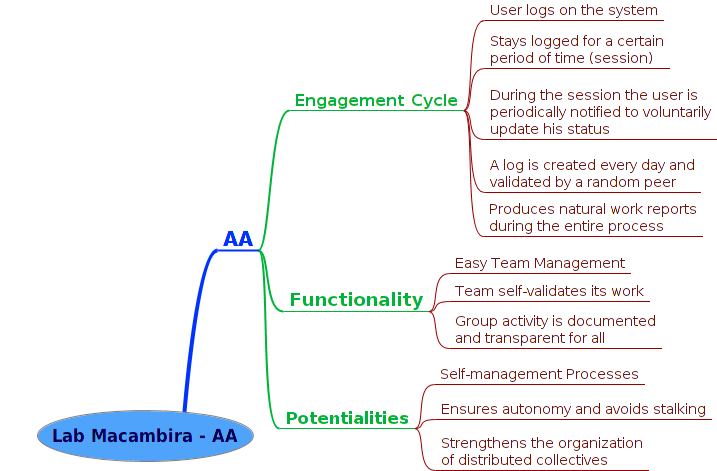
\includegraphics[width=\textwidth]{figs/aaFirstMethodology}
    \caption{A mind map of the AA methodology shared by users: i) Engagement cycle – the usage of AA; ii) Functionality – the design goals of the system; iii) Potentialities – envisioned benefits of AA by authors of the diagram. As seen in Section~\ref{sec:start}, core benefits emanate from the self-transparency aspect of~\aab, with worthy mentions to proving dedications and sharing processes.} 
    \label{fig:consult}
\end{figure}




\section{Use practices}\label{sec:use}
%\addcontentsline{toc}{subsection}{Systematic use proposals}
%tags, slots, spacing, scattered, etc. Offline
Distinct use methods are incident, mostly regarding the design exposed in \sectionb~\ref{sec:desf}. Even those cases which are not standard can be understood in the light of \aab\ paradigm. Deviations from the ideal case is always present (\sectionb~\ref{sec:devia}).

\subsection{Words and tags}\label{sec:usewt}
Throughout \aab\ usage, particular words and tags has been used to classify shouts. Of particular interest are:
\begin{itemize}
    \item Hashtags, such as \#aa, \#coding and \#articulation. These were inherited from Twitter practice. 
    \item Tags starting with ``+'' sign, such as +django, +sna and +reading. These aimed at particular used of tagging within \aab, with independence of other systems and easing concurrent use of \aab\ and other social networks.
    \item Words and abbreviations. Sometimes used in the beginning of shouts, others on the end of them, these also had the purpose of easing categorization of the shouts. These cases sometimes were pointed as tags for entire sessions or for all shouts since tagging, until another tagging shout was sent by the user.
\end{itemize}

These tagging schemes was also used as a way to enable the ``ubiquitous \aab'', i.e. usage of \aab\ in any social network or communication protocol. The \#aao0 tag was used for Twitter streaming \aab\ shouts to a considered database as is the most prominent ubiquitous \aab\ manifestation. Facebook tagging was also used to indicate posts and comments that were \aab\ shouts. On some extreme cases, tagging was used in any platform, considering ubiquitous \aab\ implemented, but not yet mined.

\subsection{Messages}\label{sec:usesh}
Messages for \aab\ usage can be of various types, as shown in Table~\ref{tab:msgTy}. Usually, the type was dictated by first word of the message. Start messages started an \aab\ session, while stop messages finished an ongoing session. Push messages sent local \aab\ sessions (or independent shouts) to a shared database. There was only one automatic message, designated to register ``lost timeslot'' of sessions (see Section~\ref{sec:usess}). Additional messages were dedicated to query for tickets attributed to the user, milestones and other traditional software development managements facilities.

\subsubsection{Shouts}
By far the most important \aab\ related message to date is the ``shout''. Dedicated to expose ongoing tasks, shouts are recurrently envisioned as a structured message, in which the user classifies the shout through special words and tags, and add a natural language description of what is being done. Nevertheless, shouts are used by all \aab\ users as a short natural language description of what current efforts, without classification whatsoever of the message. Example of structured shout proposals are in~\cite{aaWiki} and~\cite{aaREADME}.

\subsection{Sessions}\label{sec:usess}
\subsection{Developments}\label{sec:usedev}
\subsection{Suplimentary commands}\label{sec:usesc}
\subsection{Deviations from \aab\ paradigm}\label{sec:devia}

 \section{Software support}\label{sec:sofsup}
%\addcontentsline{toc}{section}{Systems and data}
 There are different software support for \aab\ (Section~\ref{sec:ss}). Also,  This section exposes this diversity and their integration, as linked data, both within \aab\ variants and within participatory instances.

There are mainly three software pieces written to support \aab\ activity. Two of them are a server and client suite each (see Sections~\ref{sec:aaFirst} and~\ref{sec:aa01}). The third is a fancy dashboard. Automated conversational agents (software [ro]bots) were used as alternative User Interfaces (\ui s), with a highlight for the Lalenia bot (see Section~\ref{sec:lalenia}), and an initiative to make \aab\ available in all chat networks (see Section~\ref{sec:ubi}).

All \aab\ software apparatus is contextualized in Table~\ref{tab:aas}.
\subsubsection{First \aab: \httpb\ server, \html\ skin and shell client}\label{sec:aaFirst}
Although deprecated in favor of \aab\ 01, this first \aab\ software presents the most numerous set of functionalities. Client functionalities are:
\begin{itemize}
    \item 
\end{itemize}

Server functionalities are:
\begin{itemize}
    \item
\end{itemize}

Core \html\ skin functionalities are:
\begin{itemize}
    \item
\end{itemize}


Further information of this and other versions of \aab\ are contextualized in Table~\ref{tab:aas}.
\subsubsection{\paaineli}\label{sec:aaFirst}
\subsubsection{\aai\ 01}\label{sec:aa01}
\subsubsection{Lalenia interface}\label{sec:lalenia}
\subsubsection{Ubiquitous \aab}\label{sec:ubi}

%\addcontentsline{toc}{subsection}{Software support}
\begin{table}[!h]
  \centering
  \caption{All considered \aab\ versions and their databases. References marked with $\dagger$ are not operational anymore.}\label{tab:aas}
  \begin{tabular}{|l|l|l|l|l|l|}\hline
      {\bf version name} & {\bf main language} & {\bf user interface} & {\bf database} & {\bf git} & {\bf available at} \\\hline\hline
& & & & & \\\hline
& & & & & \\\hline
& & & & & \\\hline
& & & & & \\\hline
& & & & & \\\hline
& & & & & \\\hline
& & & & & \\\hline
& & & & & \\\hline
& & & & & \\\hline
& & & & & \\\hline
& & & & & \\\hline
& & & & & \\\hline
  \end{tabular}
\end{table}

\subsubsection{The \#labmacambira@Freenode \irc\ channel log}
\subsubsection{Auxiliary scripts}
Python script at~\cite{mysqlTri} outputs \rdf\ from a \mysql\ database, mostly from first \aab\ version.
Python script at~\cite{mongoTri} transcribes a \mongodb\ database, mostly from first \aab\ version, to \rdf\ data.

\section{Data}\label{sec:data}
\subsection{The \ontologiaa\ \owl\ ontology}
%\addcontentsline{toc}{subsection}{The \ontologiaa\ \owl\ ontology}

\subsection{\rdfi\ data}
%\addcontentsline{toc}{subsection}{\rdfi\ data}

\subsection{Linkage to other participatory data}
%\addcontentsline{toc}{subsection}{Linkage to other participatory data}


\section{Statistics}\label{sec:stats}
%\addcontentsline{toc}{section}{Data statistics}
\subsection{Occurrent activity}

\begin{table}[!h]
  \centering
  \caption{Registered \aab messages. Operational messages, for signaling session start, stop and publishing local logs (push) are the least abundant. Usage messages with quasi-null semantic content delivers indicative that the user is connected to \aab, but no more than that. Messages registering user processes were found to be 34770+1654 = 36424. There were 7504 \irc\ \aab\ messages, of which 1654 were not registered in databases, probably because of software failures. Automated messages of `lost timeslot' are the most numerous, with almost half of all messages. }\label{tab:msgTy}
  \begin{tabular}{|l|l|l|}\hline
      {\bf message content } & {\bf count} & {\bf type}   \\\hline\hline
 push & 1718 & \multirow{3}{*}{operational messages = 3936 } \\ 
start & 1169 & \\ 
 stop & 1049 & \\ \hline\hline
 empty shouts & 92    & \multirow{3}{*}{void messages = 17125} \\
 empty alerts & 83        &  \\
       notify & 16950     &  \\ \hline\hline
      message shouts & 34770 & \multirow{2}{*}{messages about ongoing tasks = 36424}  \\ 
      \irc\ message shouts & 1654 & \\ \hline
      lost timeslot & 59863 & client automated message \\ \hline\hline
      {\bf total} & 115694 & all messages are textual \\\hline
  \end{tabular}
\end{table}


\begin{table}[!h]
  \centering
  \caption{Registered \aab sessions.}\label{tab:session}
  \begin{tabular}{|l|l|}\hline
      {\bf description} & {\bf value}   \\\hline\hline
      number of sessions & 7288 \\ \hline
      number of shouts in sessions & 20299 \\ \hline
      number sessions with more than 1 shout & 905 \\ \hline
      number of shouts in sessions with more than 1 shout & 13916 \\ \hline
      number of users in sessions & 14 \\ \hline
      number of checkers in sessions & 36 \\ \hline
      number of screencasts in sessions & 295 \\ \hline
      number of scored sessions & 191 \\ \hline
      average session score & 3.18 \\ \hline
      standard deviation of score & 0.74 \\ \hline
      average number of shouts per session & 15.38 \\ \hline
      standard deviation of number of shouts & 19.82 \\ \hline
      first session from & 2011-07-06T03:23:05 \\ \hline
      last session from & 2014-04-01T09:11:36 \\ \hline

  \end{tabular}
\end{table}


\subsubsection{Time activity}
\begin{figure}[H]
    \hspace{-25mm}
    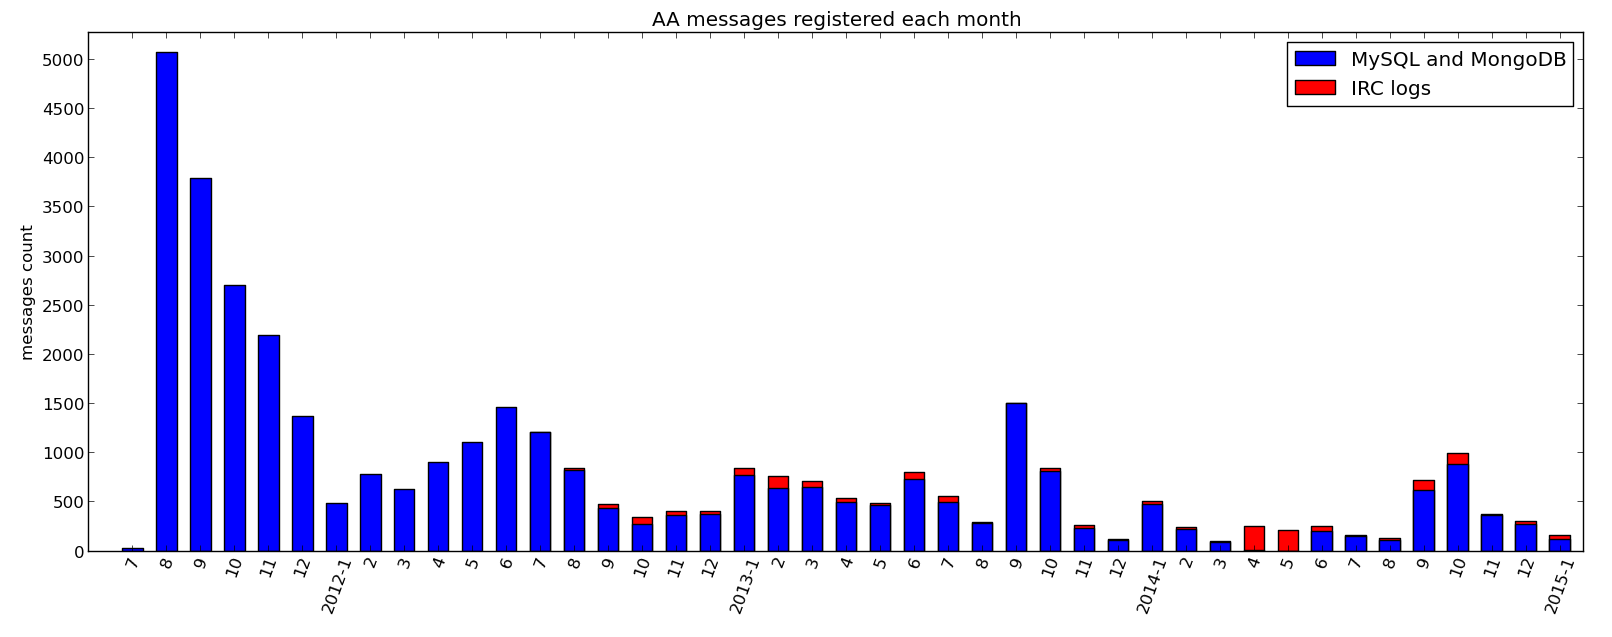
\includegraphics[width=1.3\textwidth]{imgs/actHist}
  \caption{\small The average number of messages each month is $\mu=507.1$, with a standard deviation of $\sigma=336.63 $.}\label{fig:telao2}
\end{figure}

% medida de atividade nos segundos, minutos, horas, dias da semana e do mes. Meses do ano.


\begin{figure}[H]
    \hspace{-25mm}
    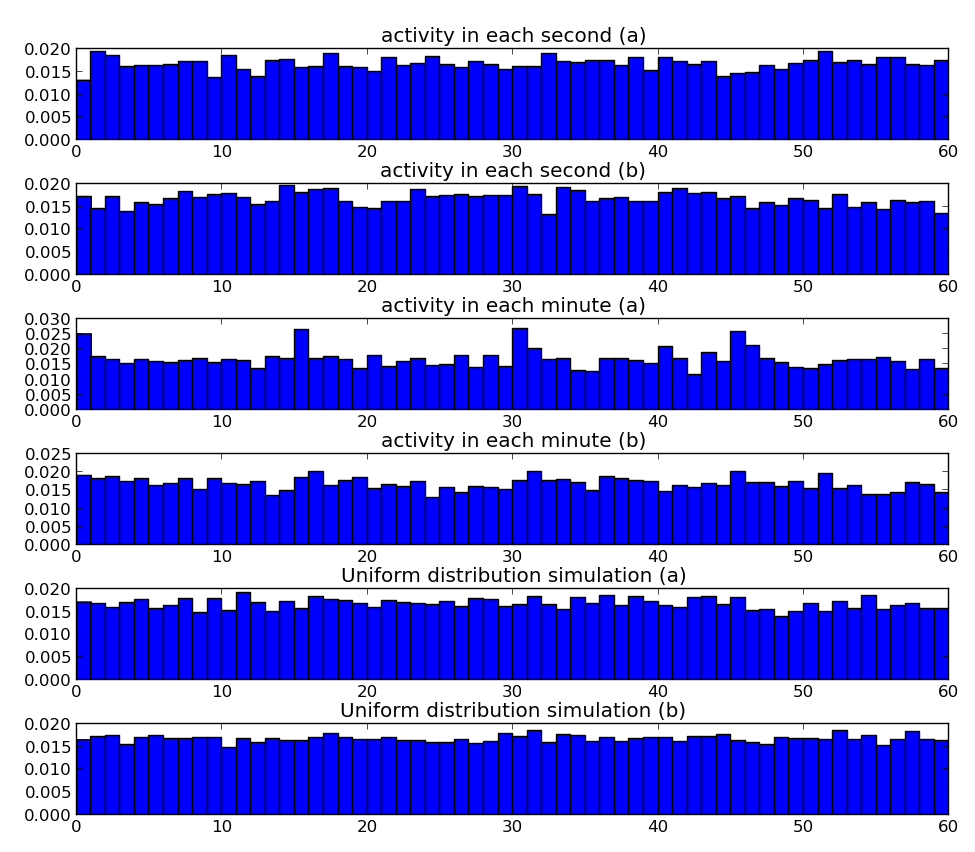
\includegraphics[width=1.3\textwidth]{imgs/segMinHist}
    \caption{\small Histogram of activity in \aab\ along seconds and minutes. A strong 15 minutes pattern is visible in (a). The same pattern is apparent in all present histograms, although less incisive. This pattern was not found in mailing lists~\cite{stabNet}, where distribution of activity along seconds and minutes was more homogeneous than Numpy uniform distribution simulator. In \aab\ the scene is the opposite: while simulations delivers $\tau=\frac{max[count(i)]}{min[count(i)]}\approx1.38$(a) and $\approx 1.26$ (b), shouts present $\tau=1.47$ and $\tau=1.48$, seconds for (a) and (b), and$\tau=2.32$ and $\tau=1.58$, minutes for (a) and (b). Means are considerably bellow $29.5$, which might indicate a tendency to shout messages in the beginning of minutes and hours. As these fluctuations among seconds and minutes were not observed in email lists (or other networks, as far as authors know), a hypothesis arises: the tasks at hand and the culture and socioeconomic factors makes timing more prominent. \aai\ itself is time-focused.}\label{fig:histSecMin}
\end{figure}



\subsubsection{User activity}
\subsection{Dependent activity}
\subsubsection{Character and token incidence}
\subsubsection{Time and user dependent activity}
\subsubsection{String and user dependent activity}
\subsubsection{String and time dependent activity}
\subsubsection{Morphosyntactic incidence}
\subsubsection{Time-related stability}
\subsection{Network activity}
\subsubsection{Time user networks}
% ambito no pico de atividade relaciona usuarios
% rede unipartida de usuarios relacionados

\subsubsection{Lexical user networks}
% utilização de verbetes em comum relaciona usuarios
% rede unipartida de usuarios relacionados

\subsubsection{Network measures}
% tabela com grausm forcas, clustering, betweenness, etc.

\subsubsection{Network primitive sectioning}
% diferenciação no particionamento das diferentes redes.

\subsection{Principal components formation}
\subsection{Immediate clustering}
\subsubsection{Users clustering}
% cada usuario eh um individuo
\subsubsection{Words clustering}
% cada verbete eh um individuo
\subsection{Timeslot clustering}
% cada hora do dia eh um individuo
\subsection{Comparative analysis}
\subsection{\aai, \ocd, and \participa}

\section{Results}\label{sec:res}

\section{Conclusions}\label{sec:con}
\subsection{Further work}
\subsection{Acknowledgments}

%\addcontentsline{toc}{subsection}{\ontologiaa: the \aab\ ontology}
%\begin{wrapfigure}{l}{0.4\textwidth} % Inline image example
%\begin{center}
%\includegraphics[width=0.38\textwidth]{telao1.png}
%\end{center}
%\caption{\small Telão para streaming de estruturas sociais, usado no \#arenaNETmundial, \#ocupaGOV e outras ocasiões. Tela com rede de retweets e relacionamento via hashtag e vocabulário. Atualizada a cada 10 segundos com os relacionamentos implicados pelos dos tweets mais recentes.}\label{fig:telao}
%\end{wrapfigure}

%\begin{figure}[H]
%  \centering
%    \includegraphics[width=.7\textwidth]{telao2.png}
%  \caption{\small Telão para streaming de estruturas sociais, usado no \#arenaNETmundial, \#ocupaGOV e outras ocasiões. Tela com relacionamentos de hashtags e vocabulário. Atualizada a cada 10 segundos com conteúdo dos tweets mais recentes.}\label{fig:telao2}
%\end{figure}










%----------------------------------------------------------------------------------------
%   BIBLIOGRAPHY
%----------------------------------------------------------------------------------------

%\bibliographystyle{unsrt}
%\bibliographystyle{plain}
\bibliographystyle{ieeetr}
\bibliography{ensaio}

%----------------------------------------------------------------------------------------

\end{document}
